\documentclass{article}

\usepackage{amsmath}
\usepackage{amssymb}
\usepackage{tcolorbox}
\usepackage{mathtools}
\usepackage{mathrsfs}
\usepackage{physics}
\usepackage{enumitem}
\usepackage{bm}
\usepackage{bbm}


\usepackage[margin=1.1in]{geometry}
\title{Error bounds of an elliptic PDE}
\date{}

\setlength\parindent{0pt}
\begin{document}
    \maketitle
    \subsection*{Introduction}
    Our goal for this project is to give accurate error bounds for approximated solutions of a problem described by an elliptic PDE. In this project we are working with the steady-state of the heat equation, which purpose is modeling how a quantity such as heat diffuses through a given region. The heat equation was first developed by Fourier studying how thermal conduction works, while the steady-state heat equation (not dependent on time, $\frac{\partial u}{\partial t} = 0$ ) of a volume that contains a heat source is described by Poisson's equation:
    \begin{align*}
        \bm{q} = -k \nabla ^2 u
    \end{align*}
    where 
    \begin{enumerate}
        \item[] $\bm{q}$ is the heat flux of the source,
        \item[] $k$ is the materials' thermal conductivity,
        \item[] $u$ is the temperature.
    \end{enumerate}

    In general terms, it states that the rate of heat transfer through a material is proportional to the negative gradient in the temperature and to the area through which the heat flows. With the previous PDE we will look at the flow rates or fluxes of energy locally. \\
    Our work will be done in 1-D and 2-D for different concrete cases. In the 1D case, Poison's equation is of the following way:
    \begin{align*}
        &\frac{\partial q}{\partial x} = f \\
        &q = -k \frac{\partial u}{\partial x} 
    \end{align*}
    And we will consider the following situations:
    \begin{enumerate}
        \item Linear flux ($\frac{\partial q}{\partial x} = 1$) and constant thermal conductivity ($k=1$).
        \item Linear flux and thermal conductivity not constant.
        \item Flux non-linear ant thermal conductivity not constant.
    \end{enumerate}

    Meanwhile, in the 2-D case we will work with:
    \begin{align*}
        &\frac{\partial q}{\partial x} + \frac{\partial q}{\partial y}  = f \\
        &\bm{q} = -k \left( \frac{\partial u}{\partial x} + \frac{\partial u}{\partial y}\right)
    \end{align*}
    But we will only consider a case where flux is linear ant the thermal conductivity is constant.
    
    \subsection*{Error bounds computations}
    Our main goal is for an approximated solution $v$, check how good it is compared to the real solution $u$ but without knowing it. The idea is that instead of measuring $\norm*{u-v} = \norm*{e_v}$ (which is the more natural way of measuring the error between both solutions), we will try to give an upper bound (called majorant) of $\norm*{k^{\frac{1}{2}}\nabla e_v}$ (This is called the error in the energy norm). By integrating the PDE and some more computations we obtain:
    \begin{align*}
        \norm*{k^{\frac{1}{2}}\nabla e_v} \leq \norm*{k^{-\frac{1}{2}}(\bm{r}+k\nabla v)} + C_{\Omega,k}\norm*{f-\nabla \bm{r}} \equiv \mathcal{M}(v,r;f)
    \end{align*}
    where $\bm{r}$ is an approximation to the flux function.
    With this error bound, one may ask hisself how can we trust the approximated solution: we may check that the majorant is "small", but to measure that "small" quantity we consider the relative error:
    \begin{align*}
        \frac{\norm*{k^{\frac{1}{2}}\nabla e_v}}{\norm*{k^{\frac{1}{2}}\nabla v}} \leq \frac{\mathcal{M}(v,r;f)}{\norm*{k^{\frac{1}{2}}\nabla v}}
    \end{align*}
    Also, in order to determine the quality of the error bound we will compute (when we do know the real solution, of course) the efficiency index, that measures how close is the error bound to the true error. For the energy error of the potential we will have:
    \begin{align*}
        I_v = \frac{\mathcal{M}(v,r;f)}{\norm*{k^{\frac{1}{2}}\nabla e_v}}
    \end{align*}
    We know, that for the case of the majorant this index will be bigger or equal to 1: the closest to 1 we are, the better we are doing.\\
    On the other hand, if we want to consider both energy error of the potential and of the flux, we can compute what is called the combined efficiency index, defined as follow:
    \begin{align*}
        I_{v;r} = \frac{3\mathcal{M}(v,r;f)}{\norm*{(e_v, e_r)}_*}
    \end{align*}
    Where the norm used in the previous equality is one chosen to measure both errors at the same time and defined the following way:
    \begin{align*}
        \norm*{(e_v,e_r)}_{*} \equiv \norm*{k^{\frac{1}{2}}\nabla e_v} + \norm*{k^{-\frac{1}{2}}e_r} + C_{\Omega,k}\norm*{\nabla e_r}
    \end{align*}
    
    And indeed, we can prove with the previous concepts that 
    \begin{align*}
        \mathcal{M}(v,r;f) \leq  \norm*{(e_v,e_r)}_{*}  \leq 3\mathcal{M}(v,r;f)
    \end{align*}

    That in terms of the efficiency index:
    \begin{align*}
        1 \leq I_{v;r} = \frac{3\mathcal{M}(v,r;f)}{\norm*{(e_v, e_r)}_*} \leq 3
    \end{align*}

    One thing to take into consideration is, because the way the Poincaré constant is defined:
    \begin{align*}
        C_{\omega,k} \equiv sup_e \frac{\norm*{e}}{\norm*{k^{\frac{1}{2}}\nabla{e}}}
    \end{align*}
    We can obtain that for any function $e$ it always will hold:
    \begin{align*}
        \norm*{e} \leq C_{\Omega,k}\norm*{k^{\frac{1}{2}}\nabla{e}} \leq C_{\Omega,k}\mathcal{M}(v,r;f)
    \end{align*}
    With this result we can really give an upper bound for the quantity we were trying to measure.

    So these are the computations that we will check for our concrete cases. But first, let us talk about the method used to do the computations:
    \subsection*{Implementation of the method}
    In our concrete problem we will be working in the unit square (unit interval in the case of 1D): we will divide it in cells, with its correspondent surrounding edges (all cells and edges numbered following a concrete order). For each cell, we will approximate the potential ($v_h \approx u$) by just evaluating the potential in the middle of the cell and assuming that is the potential in the whole cell. For the flux, we can compute an approximation ($r_h$) in every edge surrounding the cell using finite difference: $r_h^j = \pm k^j \frac{v_h^{i_1}- v_h^{i_2}}{\Delta x}$. Interpolating both flux and potential we can then obtain functions smooth enough to work with them and apply all the mentioned before.
    This is done as showed in the picture: for inner cells it is a simple interpolation cause we have all potential and fluxes needed, but for borders it is more complicated. We will rely on the following results for borders that are not corners:

    If we are considering the 1D case, following the conservation law for cell $i$ we have:
    \begin{align*}
        q_{i+1} - q_i =  \int_{w_i} f
    \end{align*}

    This can be applied the same way in the 2D case, component by component. For the particular case considered in our drawing we would have that the flux y the y-component is an interpolation between $F_T$ and $F_B$, while for the flux in the component x we need to compute $F_L$, and that is done following the previous said about the conservation law:
    \begin{align*}
        F_L &= F_R - \int\limits_{x_1}^{x_2} f(x,y) \,dx\ \\
        &=  F_R - f(x,y)\Delta x \quad \text{(Cause we are considering f being constant)}
    \end{align*}

    The remaining cells are then the corners. For that suppose our approximated flux looks like this:
    \begin{align*}
        r(x,y) = \begin{bmatrix}
            b_1+b_2*x\\
            b_3+b_4*y
            \end{bmatrix}
    \end{align*}
    Then, following the PDE, it must be satisfied that:
    \begin{align*}
        r_x + r_y &= f \quad \text{\scriptsize{(Remember we were considering f constant)}}\\
        b_2 + b_4 &= f \quad \text{\scriptsize{(First condition)}}
    \end{align*}
    On the other hand, we know that for inner edges, the flux is set to zero, so by that we are adding two more conditions. The one condition left for our 4 unknowns values is assuming $b_1 = b_3$. As we are approximating, we can totally assume this to make computations more easily. 

    \subsection*{Results in 1D}
    Once we have explained the procedure, let us dive in the numerical results.

    \subsection*{Results in 2D}
    First thing we will check is the convergence of our method. As we know the real solution, we are computing the real error with our approximated solution. As we would expect, when we do decrease the size of each step (both x and y cause are the same), the error is less. This makes sense cause the approximations we are making are more accurate as we have more "boxes" with different data to approximate. The convergence is of order 2 as one can see in the graph:
    In the graph we are plotting in a scale log log, so for knowing the order of convergence we just have to check the slope of the line we are plotting. As a comparison we have plotted too a line with a slope m = 2.
    \begin{center}
        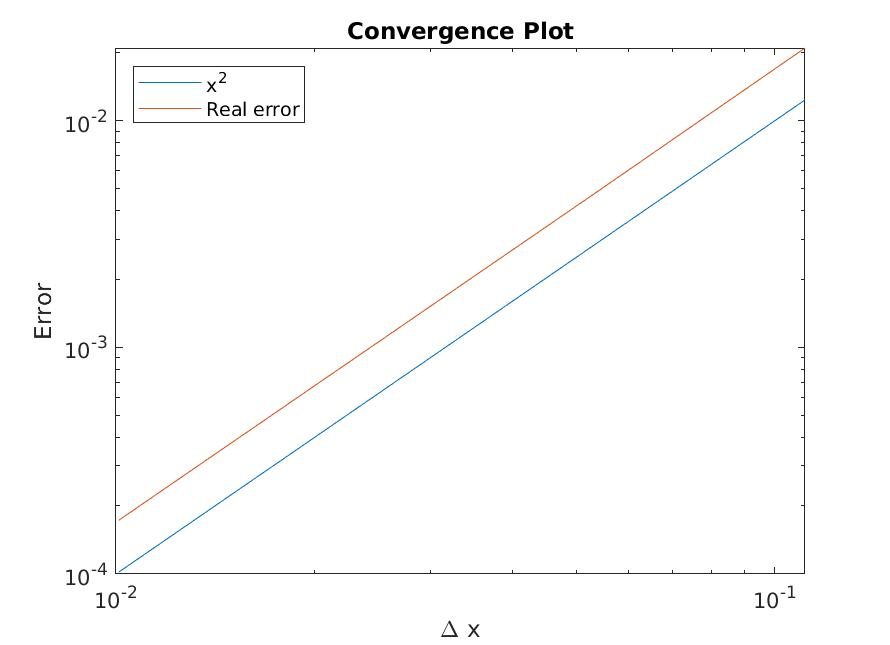
\includegraphics[width = 0.7\linewidth]{../Images/convergence2d.jpg}
    \end{center}

    Indeed, with this we can conclude that the order of convergence of our method is 2. Once we knew that, we start computing all previously mentioned. For that, see the following table where we can appreciate all inequalities we talked before:
    \begin{table}[h!]
        \centering
        \begin{tabular}{c | c | c | c | c | c }
            $\zeta$ & $\mathcal{M}$  & $\norm*{k^{\frac{1}{2}}\nabla e_v}$ & $\norm*{(e_v,e_r)}_{*}$ & $I_v^{eff}$ & $I_{v,r}^{eff}$ \\
            \hline \hline
            $\zeta_1$ (4) & 2.61 & 6.36e-1 & 2.99 & 4.10 & 2.62 \\ 
            $\zeta_2$ & 1.25 & 2.95e-1 & 1.43 & 4.26 & 2.63 \\
            $\zeta_3$ & 6.19e-1 & 1.43e-1& 7.03e-1 & 4.31 & 2.64 \\
            $\zeta_4$ & 3.07e-1 & 7.10e-2 & 3.48e-1 & 4.32 & 2.64 \\
        \end{tabular}
        \caption{2D - computations}
    \end{table}
    
    Indeed, one can easily check that the values of the combined efficiency index are between 1 and 3. Also we notice that the potential efficiency index tends to be a value of 4.3, which is not very good taking into consideration that the best we could get is 1. 
    For seeing other inequalities more clearly we show in the following graph some quantities in the table, there one can se that indeed, the norm star is between the majorant and 3majorant, that the majorant is always bigger than the real error... etc.
    \begin{center}
        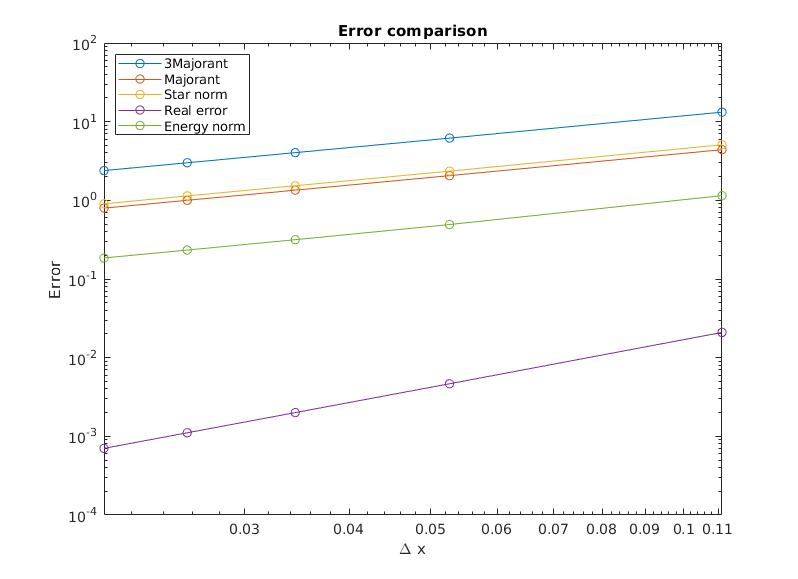
\includegraphics[width = 0.7\linewidth]{../Images/errorcomparison2d.jpg}
    \end{center}



    \subsection*{Conclusion}
    We have done computations for problems where we do know the real solution, to conclude I would like to consider a case where we do not know this real solution. Would our bound be good? We obviously can check that with the relative error, but nevertheless, it would measure how close it is to the approximated solution, not to the real solution. That's the reason why we use the efficiency index. With this last computation we have both a majorant and minorant of the efficiency index, the problem is that we need the real solution for computing the efficiency index. The conclusion then is that the ideal case would be if we have both a majorant and minorant of the quantity we are trying to measure. This way we could know how wide is our range of values for that quantity. If that range is small, we know that both minorant and majorant are giving a good bound. But in the case it is very large, we can not really tell anything about the data. (Example of our domain with our bound)
    \subsection*{References}
    All notes from INF264, code from Erlend, wikipedia

\end{document}